\documentclass[compress]{beamer}

\usepackage[nofonts]{ctex}
\setCJKmainfont[ItalicFont={Kaiti SC}]{Kaiti SC}%
%\setCJKmainfont[ItalicFont={AR PL KaitiM GB}]{AR PL KaitiM GB}%
%\setCJKsansfont{WenQuanYi Zen Hei}% 文泉驿的黑体

\mode<beamer>
{
     \useinnertheme{rectangles}
     %\useoutertheme{infolines}
     %\useoutertheme{split}
     \usecolortheme{rose}
     \usecolortheme{seahorse}

     \setbeamertemplate{navigation symbols}{}%remove navigation symbols

     %\expandafter\def\expandafter\insertshorttitle\expandafter{%
     %\insertshorttitle\hfill%
     %\insertframenumber\,/\,\inserttotalframenumber}
     %\raisebox{-1ex}{
\includegraphics[width=3ex]{Overlays/logo.pdf}}}

    \setbeamertemplate{footline} {
      \leavevmode%
      \hbox{%
      \begin{beamercolorbox}[wd=.1\paperwidth,ht=2.25ex,dp=1ex,left]{date in head/foot}%
        \usebeamerfont{date in head/foot}%
        \hspace*{1ex}\raisebox{-0.8ex}{
\includegraphics[width=3ex]{Overlays/logo.pdf}}%
      \end{beamercolorbox}%
      \begin{beamercolorbox}[wd=.4\paperwidth,ht=2.25ex,dp=1ex,right]{date in head/foot}%
        \usebeamerfont{date in head/foot}\insertsection\hspace*{1ex}
      \end{beamercolorbox}%
      \begin{beamercolorbox}[wd=.4\paperwidth,ht=2.25ex,dp=1ex,left]{date in head/foot}%
        \usebeamerfont{date in head/foot}\hspace*{1ex}\insertsubsection
      \end{beamercolorbox}%
      \begin{beamercolorbox}[wd=.1\paperwidth,ht=2.25ex,dp=1ex,right]{date in head/foot}%
        \insertframenumber{} / \inserttotalframenumber\hspace*{1ex}
      \end{beamercolorbox}}%
      \vskip0pt%
    }

}

%\defbeamertemplate*{footline}{mytheme}
%{
%  \leavevmode%
%  \hbox{%
%  \begin{beamercolorbox}[wd=.5\paperwidth,ht=2.25ex,dp=1ex,center]{author in head/foot}%
%    \usebeamerfont{author in head/foot}\insertshortauthor~~%
%    \raisebox{-1ex}{
\includegraphics[width=3ex]{Overlays/logo.pdf}}%
%  \end{beamercolorbox}%
%  \begin{beamercolorbox}[wd=.5\paperwidth,ht=2.25ex,dp=1ex,right]{title in head/foot}%
%    \usebeamerfont{title in head/foot}\insertshorttitle{}\hspace*{2em}
%    \insertframenumber{} / \inserttotalframenumber\hspace*{2ex} 
%  \end{beamercolorbox}}%
%  \vskip0pt%
%}
%\usebeamertemplate{mytheme}

%\setbeamercovered{transparent}

\mode<handout>
{
	\usetheme{default}
	\usepackage{pgfpages}
	\pgfpagesuselayout{4 on 1}[a4paper,landscape,border shrink=5mm]
}


\usepackage{amsmath,latexsym,amssymb,amsfonts,amsbsy}
\usepackage{graphicx}
\usepackage{array}
\usepackage{hyperref}
\usepackage{listings}
\usepackage{fancyvrb}
\fvset{frame=single, numbers=left, fontsize=\small}
%\usepackage{alltt}
\usepackage{textpos}
\usepackage{ulem}
\usepackage{boxedminipage}
\usepackage{comment}
\usepackage{tikz}
\usetikzlibrary{calc,arrows.meta, graphs, trees, shapes, positioning, decorations.markings, intersections, decorations.text}
\usepackage{tikz-uml}

\newcommand{\romannumber}[1]{{\textrm{\uppercase\expandafter{\romannumeral
#1}}}}

\setbeamercolor{dblue}{fg=white,bg=gray!70!blue} % for beamercolorbox
 \newenvironment{pblock}{\begin{beamercolorbox}[rounded=true,
          shadow=false]{dblue}}{\end{beamercolorbox}}
 \newenvironment{bblock}{\begin{beamercolorbox}[rounded=true,
          shadow=false]{fg=black, bg=white}}{\end{beamercolorbox}}

\graphicspath{{figure/}}

\lstset{
	basicstyle=\footnotesize\ttfamily, % print whole listing footnotesize
	keywordstyle=\footnotesize\color{black}\ttfamily\bfseries, 
	identifierstyle=\footnotesize\color{blue}\ttfamily, 
	commentstyle=\footnotesize\itshape\ttfamily, 
	stringstyle=\footnotesize\ttfamily,
	frame=single, 
	numbers=left, numberstyle=\tiny,
	stepnumber=1, numbersep=10pt,
	showtabs=false, tabsize=4,
	showstringspaces=false,
	breaklines=true, breakatwhitespace=true,
	language=[ISO]C++
}   

 
%%%%%%%%%%%%%%%%%%%%%%%%%%%%%%%%%%%%%%%%%%%%%%%%%%%%%%%%%%%%%%%%%
%    body                                                       %
%%%%%%%%%%%%%%%%%%%%%%%%%%%%%%%%%%%%%%%%%%%%%%%%%%%%%%%%%%%%%%%%%


\begin{document}

\AtBeginSubsection[]
{ 
    \begin{frame}<beamer> 
		\frametitle{内容提要} 
		\tableofcontents[currentsection,currentsubsection,
        subsectionstyle=show/shaded/hide] 
	\end{frame} 
} 

					
\title{第七章 ~~ 面向对象的系统设计\MakeUppercase{\romannumeral 1}}

\author[面向对象的分析与设计]
{曹东刚\\\href{mailto:caodg@pku.edu.cn}{caodg@pku.edu.cn}}

\institute[北京大学]{北京大学信息学院研究生课程 - 面向对象的分析与设计 \\
\href{http://sei.pku.edu.cn/~caodg/course/oo}{http://sei.pku.edu.cn/\~{}caodg/course/oo}}

\date{}

\titlegraphic{
\includegraphics[height=0.10\textwidth]{Overlays/logo.pdf}}

\begin{frame}[plain]
	\titlepage
\end{frame}

\setcounter{framenumber}{0}

\section{OOD概览}

\begin{frame}
\frametitle{OOD框架---两个侧面}

\begin{columns}

\column{0.3\hsize}

\begin{itemize}
\item OOD模型包括几个主要部分?
\item OOD模型每个部分如何用OO概念表达?
\end{itemize}

\column{0.7\hsize}

%\resizebox{0.6\hsize}{!}{
\begin{tikzpicture}
\renewcommand\baselinestretch{1.0}
%\draw [help lines, step=0.5cm] (-4,0) grid (6,6) ;

\draw [very thick] (0,0) -- (5,0) -- (5,5) -- (0,5) -- (0,0) ;
\draw (0,0) -- (1,1) -- (1,5);
\draw (5,0) -- (4,1) -- (4,5);
\draw (1,1) -- (4,1) ;
\node [text width=1pt] at (0.4,3.0) {人机交互部分} ;
\node [text width=1pt] at (4.4,3.0) {数据接口部分} ;
\node at (2.5,0.5) {控制驱动部分} ;
\node at (2.5,3.0) {\Large{问题域部分}} ;

\draw [very thick](0,0) -- (-3,1) --(-3,6) ;
\draw [name path=c2, very thick] (-3,6) -- (0,5) ;
\draw [name path=c1, postaction={decorate, decoration={text along path, raise=-15pt, text align={align=center}, text = {模型规约}}}] (-3,2) -- (0,1) ;

\draw [very thick](5,5) -- (2,6)--(-3,6) ;
\path [name path=v1] (-0.75,0) -- (-0.75,6) ;
\path [name path=v2] (-2.25,0) -- (-2.25,6) ;

\path [name intersections={of=c1 and v1,by=E1}];
\path [name intersections={of=c2 and v1,by=E2}];
\draw (E1) -- (E2) ;
\path [name intersections={of=c1 and v2,by=F1}];
\path [name intersections={of=c2 and v2,by=F2}];
\draw (F1) -- (F2) ;

\node [text width=1pt] at (-2.75, 4) { 需求模型} ;
\node [text width=1pt] at (-0.5, 3) { 辅助模型} ;
\node [text width=1pt] at (-1.75, 3.5) { \Large 类图} ;

\end{tikzpicture}
%}

\end{columns}
\end{frame}

\begin{frame}
\frametitle{OOD过程}
\noindent\begin{tikzpicture}[thick]
\tikzstyle{vecArrow} = [thick, decoration={markings,mark=at position
   1 with {\arrow[thin, scale=2]{open triangle 60}}},
   double distance=3pt, shorten >= 10pt,
   preaction = {decorate},
   postaction = {draw,line width=3pt, white,shorten >= 9pt}
]
\tikzstyle{Node} = [thick, rectangle, draw, minimum height=3ex, minimum width=3.5cm]

  \node (ooa) {\textcolor{blue}{输入OOA模型}};
  \node [Node, below = 1cm of ooa] (business) {问题域部分设计};
  \node [Node, below = 1cm of business] (control) {控制驱动部分设计};
  \node [Node, below = 1cm of control] (deploy) {构件化与系统部署} ;
  \node [below = 1cm of deploy] (oop) {\textcolor{blue}{向OOP输出OOD模型}} ;
  \node [Node, right = 0.5cm of control.east] (data) {数据接口部分设计};
  \node [Node, left = 0.5cm of control.west] (gui) {人机交互部分设计};

  \draw[vecArrow] (ooa) to (business);
  \draw[vecArrow] ([yshift=-1pt]business.south) to (control);
  \draw[vecArrow] ([yshift=-1pt]control.south) to (deploy);
  \draw[vecArrow] ([yshift=-1pt]deploy.south) to (oop);
  \draw[vecArrow] ([xshift=-1.0cm, yshift=-0.1cm]business.south) to ([yshift=+0.1cm]gui.north);
  \draw[vecArrow] ([xshift=+1.0cm, yshift=-0.1cm]business.south) to ([yshift=+0.1cm]data.north);
  \draw[vecArrow] ([yshift=-0.1cm]gui.south) to ([xshift=-1cm, yshift=+0.1cm]deploy.north);
  \draw[vecArrow] ([yshift=-0.1cm]data.south) to ([xshift=+1cm, yshift=+0.1cm]deploy.north);
\end{tikzpicture}

\end{frame}

\section{问题域部分的设计}

\subsection{简介}

\begin{frame}
\frametitle{什么是问题域部分}

问题域部分是OOD模型的四个组成部分之一,由来自问题域的对象构成,是在OOA模型基础上,按照具体的实现条件进行必要的修改、调整和细节补充而得到的 \\[2ex]

\resizebox{0.8\hsize}{!}{
\begin{tikzpicture}
\renewcommand\baselinestretch{1.0}
\draw [very thick] (0,0) -- (5,0) -- (5,5) -- (0,5) -- (0,0) ;
\draw (0,0) -- (1,1) -- (1,5);
\draw (5,0) -- (4,1) -- (4,5);
\draw (1,1) -- (4,1) ;
\node [text width=1pt] at (0.4,3) {人机交互部分} ;
\node [text width=1pt] at (4.4,3) {数据接口部分} ;
\node at (2.5,0.5) {控制驱动部分} ;
\node at (2.5,3) {\Large{问题域部分}} ;

\node (Impl) [rectangle, draw, text width=4cm] at (8,6) { 编程语言、网络、操作系统、复用支持等实现条件}  ;

\node (OOA) [rectangle, align=center, draw , thick] at (-2,6) {\Large OOA \\ \Large 模型}  ;

\draw [arrows= {-Triangle[angle=120:3pt 1]}, line width=0.5cm, draw=gray] (Impl)--(4,6) arc (90:160:1cm) -- (3,5) ;
\draw [arrows= {-Triangle[angle=120:3pt 1]}, line width=0.5cm, draw=gray] (OOA)--(1,6) arc (90:20:1cm) -- (2,5) ;
\end{tikzpicture}
}

\end{frame}

\begin{frame}
\frametitle{实现条件对问题域部分的影响}

\begin{itemize}
\item 编程语言
\begin{itemize}
\item 语言的实现能力
\end{itemize}
\item 硬件、操作系统及网络设施 
\begin{itemize}
\item 对象分布、并发、通信、性能 
\end{itemize}
\item 复用支持 
\begin{itemize}
\item 根据复用支持对模型做适当调整,以实现复用
\end{itemize}
\item 数据管理系统 
\begin{itemize}
\item 为实现对象的持久存储,对问题域部分做某些修改
\end{itemize}
\item 界面支持系统
\begin{itemize}
\item 问题域部分与人机界面之间的消息传输
\end{itemize}
\end{itemize}

\end{frame}

\begin{frame}
\frametitle{设计过程}

\only<1> {
\begin{itemize}
\item 设计准备
\begin{itemize}
\item 保留OOA文档
\item 复制OOA文档,作为OOD的输入
\begin{itemize}
\item 根据需求的变化和发现的错误进行修改
\end{itemize}
\end{itemize}
\end{itemize}
}

\only<2> {
\begin{itemize}
\item 设计内容与策略
\begin{itemize}
\item 针对编程语言支持能力的调整 
\item 增加一般类以建立共同协议 
\item 实现复用
\item 提高性能 
\item 为实现对象持久存储所做的修改 
\item 完善对象的细节 
\item 定义对象实例 
\item 对辅助模型、模型规约的修改和补充
\end{itemize}
\item 建立OOD文档与OOA文档的映射
\end{itemize}
}

\end{frame}

\subsection{设计内容}

\begin{frame}
\frametitle{1. 按编程语言调整继承与多态}
OOA强调如实地反映问题域,OOD考虑实现问题 \\[2ex]
如果语言不支持多继承或多态,就要进行对模型调整 \\[2ex]
\quad \uline{多继承化为单继承}
\end{frame}

\begin{frame}
\frametitle{多继承简单转换为单继承}

\only<1-2> {
\noindent\begin{tikzpicture}
\tikzumlset{fill class=white}
\umlemptyclass[width=6ex]{A}
\umlemptyclass[x=1, y=3, width=6ex]{B}
\umlemptyclass[x=-1, y=3, width=6ex]{C}
\umlinherit{A}{B}
\umlinherit{A}{C}
\end{tikzpicture}%
\raisebox{2cm}{\textcolor{red}{$\Longrightarrow$}}%
\begin{tikzpicture}
\tikzumlset{fill class=white}
\umlemptyclass[width=6ex]{A}
\umlemptyclass[x=1, y=3, width=6ex]{B}
\umlemptyclass[x=-1, y=3, width=6ex]{C}
\umlinherit{A}{B}
\umlaggreg[mult1=1, mult2=1, pos2=0.7]{A}{C}
\end{tikzpicture}%
}
\only<2> {
\raisebox{2cm}{\textcolor{red}{或}}%
\begin{tikzpicture}
\tikzumlset{fill class=white}
\umlemptyclass[width=6ex]{A}
\umlemptyclass[x=1, y=3, width=6ex]{B}
\umlemptyclass[x=-1, y=3, width=6ex]{C}
\umlaggreg[mult1=1, mult2=1, pos1=0.3, pos2=0.9]{A}{B}
\umlaggreg[mult1=1, mult2=1, pos1=0.1, pos2=0.7]{A}{C}
\end{tikzpicture}
}

\only<3-4> {
例子: \\[2ex]
\noindent \resizebox{0.3\hsize}{!} {
\begin{tikzpicture}
\tikzumlset{fill class=white}
\umlemptyclass[width=7ex]{冷藏车}
\umlemptyclass[x=1, y=3, width=5ex]{汽车}
\umlemptyclass[x=-1, y=3, width=9ex]{制冷设备}
\umlinherit{冷藏车}{汽车}
\umlinherit{冷藏车}{制冷设备}
\end{tikzpicture}
}%
\raisebox{2cm}{\textcolor{red}{$\Rightarrow$}}%
\resizebox{0.3\hsize}{!} {
\begin{tikzpicture}
\tikzumlset{fill class=white}
\umlemptyclass[width=7ex]{冷藏车}
\umlemptyclass[x=1, y=3, width=5ex]{汽车}
\umlemptyclass[x=-1, y=3, width=9ex]{制冷设备}
\umlinherit{冷藏车}{汽车}
\umlaggreg[mult1=1, mult2=1, pos2=0.7]{冷藏车}{制冷设备}
\end{tikzpicture}
}%
}
\only<4> {
\raisebox{2cm}{\textcolor{red}{或}}%
\resizebox{0.3\hsize}{!} {
\begin{tikzpicture}
\tikzumlset{fill class=white}
\umlemptyclass[width=7ex]{冷藏车}
\umlemptyclass[x=1, y=3, width=5ex]{汽车}
\umlemptyclass[x=-1, y=3, width=9ex]{制冷设备}
\umlaggreg[mult1=1, mult2=1, pos1=0.3, pos2=0.9]{冷藏车}{汽车}
\umlaggreg[mult1=1, mult2=1, pos2=0.7]{冷藏车}{制冷设备}
\end{tikzpicture}
}
}

\only<5> {
例子: \\[2ex]
\begin{tikzpicture}
\tikzumlset{fill class=white}
\umlemptyclass{在职学员}
\umlemptyclass[x=1, y=3]{学员}
\umlemptyclass[x=-1, y=3]{职员}
\umlinherit{在职学员}{学员}
\umlinherit{在职学员}{职员}
\end{tikzpicture}%
\begin{tikzpicture}
\tikzumlset{fill class=white}
\umlemptyclass{在职学员}
\umlemptyclass[x=1, y=3]{学员}
\umlemptyclass[x=-1, y=3]{职员}
\umlaggreg[mult1=1, mult2=1, pos1=0.3, pos=0.9]{在职学员}{学员}
\umlaggreg[mult1=1, mult2=1, pos1=0.1, pos2=0.7]{在职学员}{职员}
\node at (-2.5, 2) {\textcolor{red}{$\Longrightarrow$}} ;
\node at (-2.5, 2) {\Large ?} ;
\end{tikzpicture}
}

\only<6> {
转换产生信息重复: \\[2ex]
\resizebox{!}{6cm} {
\begin{tikzpicture}
\tikzumlset{fill class=white}
\umlemptyclass{A}
\umlemptyclass[x=1, y=-3]{B}
\umlemptyclass[x=-1, y=-3]{C}
\umlemptyclass[y=-6]{D}
\umlinherit[geometry=|-|]{B}{A}
\umlinherit[geometry=|-|]{C}{A}
\umlinherit{D}{B}
\umlinherit{D}{C}
\end{tikzpicture}%
}
\resizebox{!}{6cm} {
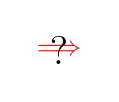
\begin{tikzpicture}
\tikzumlset{fill class=white}
\umlemptyclass{A}
\umlemptyclass[x=1, y=-3]{B}
\umlemptyclass[x=-1, y=-3]{C}
\umlemptyclass[y=-6]{D}
\umlinherit[geometry=|-|]{B}{A}
\umlinherit[geometry=|-|]{C}{A}
\umlinherit{D}{B}
\umlaggreg[mult1=1, mult2=1, pos1=0.1, pos2=0.7]{D}{C}
\node at (-2.5, -1) {\textcolor{red}{$\Longrightarrow$}} ;
\node at (-2.5, -1) {\Large ?} ;
\end{tikzpicture}
}
}

\end{frame}

\begin{frame}
\frametitle{重新定义类化解多继承}

\only<1> {
\begin{tikzpicture}
\tikzumlset{fill class=white}
\umlemptyclass{人员}
\umlemptyclass[x=1, y=-2.5]{学员}
\umlemptyclass[x=-1, y=-2.5]{职员}
\umlemptyclass[y=-5]{在职学员}
\umlinherit{职员}{人员}
\umlinherit{学员}{人员}
\umlinherit{在职学员}{学员}
\umlinherit{在职学员}{职员}
\end{tikzpicture}%
\raisebox{4.5cm}{\quad\textcolor{red}{$\Longrightarrow$}}%
\raisebox{1.5cm}{
\begin{tikzpicture}
\tikzumlset{fill class=white}
\umlemptyclass{人员}
\umlemptyclass[x=1.5, y=-2.5]{学员身份}
\umlemptyclass[x=-1.5, y=-2.5]{职员身份}
\umlaggreg[mult1=1, mult2={0..1}, pos2=0.5, pos1=0.1] {人员}{学员身份}
\umlaggreg[mult1=1, mult2={0..1}, pos1=0.5, pos2=0.95] {人员}{职员身份}
\end{tikzpicture}
}
}

\only<2> {
\begin{tikzpicture}
\tikzumlset{fill class=white}
\umlemptyclass{人员}
\umlemptyclass[x=1, y=-2.5]{学员}
\umlemptyclass[x=-1, y=-2.5]{职员}
\umlemptyclass[y=-5]{在职学员}
\umlinherit{职员}{人员}
\umlinherit{学员}{人员}
\umlinherit{在职学员}{学员}
\umlinherit{在职学员}{职员}
\end{tikzpicture}%
\raisebox{4.5cm}{\quad\textcolor{red}{$\Longrightarrow$}}%
\begin{tikzpicture}
\tikzumlset{fill class=white}
\umlemptyclass{人员}
\umlemptyclass[y=-2.5]{身份}
\umlemptyclass[x=1.5, y=-5]{学员身份}
\umlemptyclass[x=-1.5, y=-5]{职员身份}
\umlaggreg[mult1=1, mult2={0..2}]{人员}{身份}
\umlinherit[geometry=|-|]{职员身份}{身份}
\umlinherit[geometry=|-|]{学员身份}{身份}
\end{tikzpicture}
}

\end{frame}

\begin{frame}
\frametitle{保持分类,剥离多继承信息}
\begin{tikzpicture}
\tikzumlset{fill class=white}
\umlemptyclass{人员}
\umlemptyclass[x=1, y=-2.5]{学员}
\umlemptyclass[x=-1, y=-2.5]{职员}
\umlemptyclass[y=-5]{在职学员}
\umlinherit{职员}{人员}
\umlinherit{学员}{人员}
\umlinherit{在职学员}{学员}
\umlinherit{在职学员}{职员}
\end{tikzpicture}%
\raisebox{4.5cm}{\quad\textcolor{red}{$\Longrightarrow$}}%
\begin{tikzpicture}
\tikzumlset{fill class=white}
\umlemptyclass{人员}
\umlemptyclass[y=-2.5]{在职学员}
\umlemptyclass[x=-2, y=-2.5]{职员}
\umlemptyclass[x=2, y=-2.5]{学员}
\umlemptyclass[x=1.5, y=-5]{学员信息}
\umlemptyclass[x=-1.5, y=-5]{职员信息}
\umlinherit{在职学员}{人员}
\umlinherit[geometry=|-|]{职员}{人员}
\umlinherit[geometry=|-|]{学员}{人员}
\umlaggreg[mult1=1, mult2=1, pos1=0.1, pos2=0.5]{职员}{职员信息}
\umlaggreg[mult1=1, mult2=1, pos1=0.5, pos2=0.95]{在职学员}{职员信息}
\umlaggreg[mult1=1, mult2=1, pos1=0.1, pos=0.5]{在职学员}{学员信息}
\umlaggreg[mult1=1, mult2=1, pos1=0.5, pos2=0.95]{学员}{学员信息}
\end{tikzpicture}
\end{frame}

\begin{frame}
\frametitle{取消多态性}
\noindent
\resizebox{0.38\hsize}{!}{
\begin{tikzpicture}
\tikzumlset{fill class=white}
\renewcommand\baselinestretch{1.0}
\umlclass{多边形}{线条色 \\
线型 \\
边数 \\
顶点坐标}{绘图 \\
填充}
\umlclass[y=-4, x=-1.3]{正多边形}{*顶点坐标\\{}}{*绘图}
\umlclass[y=-4, x=1.3]{矩形}{*顶点坐标\\ $\times$边数}{*绘图}

\umlinherit[geometry=|-|, arm1=1.5cm]{正多边形}{多边形}
\umlinherit[geometry=|-|, arm1=1.5cm]{矩形}{多边形}
\end{tikzpicture}
}%
\pause
\raisebox{4cm}{\textcolor{red}{$\Longrightarrow$}}%
\resizebox{0.62\hsize}{!}{
\begin{tikzpicture}
\renewcommand\baselinestretch{1.0}
\tikzumlset{fill class=white}
\umlclass{多边形}{线条色 \\ 线型} {填充}
\umlclass[y=-4]{正多边形}{顶点坐标\\边数}{绘图}
\umlclass[y=-4, x=-2.7]{不规则多边形}{顶点坐标\\边数}{绘图}
\umlclass[y=-4, x=2.3]{矩形}{顶点坐标\\ {}}{绘图}

\umlinherit[geometry=|-|]{正多边形}{多边形}
\umlinherit[geometry=|-|]{矩形}{多边形}
\umlinherit[geometry=|-|]{不规则多边形}{多边形}
\end{tikzpicture}
}
\end{frame}

\begin{frame}
\frametitle{2. 增加一般类以建立共同协议}
\only<1> {
\begin{itemize}
\item 增加根类:将所有的类组织在一起,提供全系统通用的协议 \\

  \textcolor{blue}{例}:提供创建、删除、复制等操作

\item 增加其他一般类:提供局部通用的协议 \\
  \textcolor{blue}{例}:提供持久存储及恢复功能
\end{itemize}
}

\only<2>{
\resizebox{0.7\hsize}{!}{
\begin{tikzpicture}
\tikzumlset{fill class=white}
\umlclass{A}{属性}{操作}
\umlclass[x=4]{D}{属性}{操作}
\umlclass[x=6.5]{F}{属性}{操作}
\umlclass[x=4, y=-3.5]{E}{属性}{操作}
\umlclass[x=1.25, y=-3.5]{C}{属性}{操作}
\umlclass[x=-1.25, y=-3.5]{B}{属性}{操作}
\umlinherit[geometry=|-|]{B}{A}
\umlinherit[geometry=|-|]{C}{A}
\umlaggreg[mult1=1, mult2=*]{D}{E}
\end{tikzpicture}
}
}

\only<3>{
\resizebox{0.7\hsize}{!}{
\begin{tikzpicture}
\tikzumlset{fill class=white}
\umlclass{A}{属性}{操作}
\umlclass[x=4]{D}{属性}{操作}
\umlclass[x=6.5]{F}{属性}{操作}
\umlclass[x=4, y=-3.5]{E}{属性}{操作}
\umlclass[x=1.25, y=-3.5]{C}{属性}{操作}
\umlclass[x=-1.25, y=-3.5]{B}{属性}{操作}
\umlinherit[geometry=|-|]{B}{A}
\umlinherit[geometry=|-|]{C}{A}
\umlaggreg[mult1=1, mult2=*]{D}{E}
\umlemptyclass[type=复用, x=2.5, y=3.5, fill=yellow!20]{Object}
\umlinherit[geometry=|-|]{A}{Object}
\umlinherit[geometry=|-|]{D}{Object}
\umlinherit[geometry=|-|]{F}{Object}
\umlinherit[geometry=|-|, anchor1=120, weight=0.3]{E}{Object}
\end{tikzpicture}
}
}

\end{frame}


\begin{frame}
  \frametitle{3. 实现复用的设计策略}
  如果已存在一些可复用的类,而且这些类既有分析、设计时的定义,又有源程序
  ,那么,复用这些类可提高开发效率与质量 \\[2ex]
  \fbox{目标:尽可能使复用成分增多,新开发的成分减少} \\[2ex]

  可复用类定义的信息 \alert{VS} 当前所需的类的信息: \\
  \begin{tabular}{ll}
    \alert{$=$} & 直接复用 \\
    \alert{$<$} & 通过继承复用 \\
    \alert{$>$} & 删除可复用类的多余信息 \\
    \alert{$\approx$} & 删除多余信息,通过继承而复用
  \end{tabular}
\end{frame}

\begin{frame}
  \frametitle{示例}
  \only<1> {
  \begin{tikzpicture}
    \tikzumlset{fill class=white, fill note=white}
    \umlclass{车辆}{序号\\颜色\\式样\\出厂年月}{序号认证}
    \umlnote[x=-1,y=3.5, width=2.5cm]{车辆}{问题域中的类}
  \end{tikzpicture}%
  \qquad\qquad\qquad %
  \begin{tikzpicture}
    \tikzumlset{fill note=white}
    \umlclass{车辆}{序号\\厂商\\式样}{序号认证}
    \umlnote[x=1,y=3, width=2cm]{车辆}{可复用的类}
  \end{tikzpicture}
}

  \only<2> {
  \begin{tikzpicture}
    \tikzumlset{fill note=white}
    \umlclass[fill=white]{问题域车辆}{\sout{序号}\\颜色\\ \sout{式样}\\
  出厂年月}{\sout{序号认证}}
    \umlnote[x=-1,y=3.5, width=2.5cm]{车辆}{问题域中的类}
    \umlclass[x=5]{车辆}{序号\\ \sout{厂商}\\式样}{序号认证}
    \umlnote[x=6,y=3, width=2cm]{车辆}{可复用的类}
    \umlinherit{问题域车辆}{车辆}
  \end{tikzpicture}
  }
\end{frame}

\begin{frame}
  \frametitle{4. 提高性能}
  影响性能的因素 

  \begin{itemize}
      \item 数据传输时间 
      \item 数据存取时间 
      \item 数据处理时间
  \end{itemize}
\end{frame}

\begin{frame}
  \frametitle{4. 改善性能的策略}
  \only<1> {
  \begin{enumerate}
    \item 调整对象分布
  \end{enumerate}
  \resizebox{0.4\hsize}{!}{
  \begin{tikzpicture}
    \tikzumlset{fill component=white}
    \begin{umlcomponent}{Comp1}
      \umlemptyclass[width=5ex]{A}
      \umlemptyclass[x=2.5, width=5ex]{B}
      \umldep[stereo=call]{A}{B}
    \end{umlcomponent}
    \begin{umlcomponent}[y=-3.5]{Comp2}
      \umlemptyclass[width=5ex]{C}
    \end{umlcomponent}
    \umldep[geometry=|-,stereo=send]{B}{C}
  \end{tikzpicture}}%
  \quad \raisebox{3cm}{\textcolor{red}{$\Longrightarrow$}} \quad%
  \resizebox{0.4\hsize}{!}{
  \begin{tikzpicture}
    \tikzumlset{fill component=white}
    \begin{umlcomponent}{Comp1}
      \umlemptyclass[width=5ex]{A}
    \end{umlcomponent}
    \begin{umlcomponent}[y=-3.5]{Comp2}
      \umlemptyclass[width=5ex]{B}
      \umlemptyclass[x=2.5, width=5ex]{C}
      \umldep[stereo=call]{B}{C}
    \end{umlcomponent}
    \umldep[stereo=send]{A}{B}
  \end{tikzpicture}
  }
}

  \only<2> {
    \begin{enumerate}
      \setcounter{enumi}{1}
      \item 合并通讯频繁的类
    \end{enumerate}
    \begin{tikzpicture}
      \tikzumlset{fill class=white}
      \umlclass{流速调节器}{指定流速 \\ \ldots }{流速调节 \\ \ldots}
      \umlclass[x=4]{流速探测器}{当前流速 \\ \ldots }{流速探测 \\取当前
      流速\\ \ldots}
      \umldep[stereo=call]{流速调节器}{流速探测器}
    \end{tikzpicture}%
    \quad \raisebox{2cm}{\textcolor{red}{$\Longrightarrow$}} \quad%
    \begin{tikzpicture}
      \tikzumlset{fill class=white}
      \umlclass{流速控制器}{指定流速 \\ 当前流速 \\ \ldots }{流速调节 \\
      流速探测 \\ \ldots}
    \end{tikzpicture}
  }

  \only<3> {
  \begin{enumerate}
      \setcounter{enumi}{2}
  \item 细化对象的分类
  \end{enumerate}
  \raisebox{2cm}{
    \begin{tikzpicture}
      \tikzumlset{fill class=white}
      \umlclass{二次曲线}{}{绘图}
    \end{tikzpicture}
  }
    \quad \raisebox{3cm}{\textcolor{red}{$\Longrightarrow$}} \quad%
    \begin{tikzpicture}
      \tikzumlset{fill class=white}
      \umlclass{二次曲线}{}{绘图}
      \umlclass[y=-3]{抛物线}{}{绘图}
      \umlclass[x=-2, y=-3]{椭圆}{}{绘图}
      \umlclass[x=2, y=-3]{双曲线}{}{绘图}
      \umlinherit[geometry=|-|]{椭圆}{二次曲线}
      \umlinherit[geometry=|-|]{双曲线}{二次曲线}
      \umlinherit{抛物线}{二次曲线}
    \end{tikzpicture}
  }

  \only<4> {
    \begin{enumerate}
      \setcounter{enumi}{3}
      \item 将复杂对象化为整体-部分结构
    \end{enumerate}
\raisebox{2cm}{
    \begin{tikzpicture}
      \tikzumlset{fill class=white}
      \umlclass{帧}{}{显示}
    \end{tikzpicture}
  }
    \quad \raisebox{3cm}{\textcolor{red}{$\Longrightarrow$}} \quad%
    \begin{tikzpicture}
      \tikzumlset{fill class=white}
      \umlemptyclass{帧}
      \umlclass[y=-3, x=-2]{背景}{}{显示}
      \umlclass[y=-3, x=2]{前景}{}{显示}
      \umlaggreg[mult1=*, mult2=1, pos1=0.4]{帧}{背景}
      \umlaggreg[mult1=1, mult2=1]{帧}{前景}
    \end{tikzpicture}
  }

  \only<5> {
    \begin{enumerate}
        \setcounter{enumi}{4}
      \item 缩短对象存取时间,如设立缓冲区
      \item 增加属性以减少重复计算
      \item 降低算法的计算复杂性
    \end{enumerate}
  }
\end{frame}

\begin{frame}
  \frametitle{5. 为数据存储管理增补属性与操作}
    在数据接口部分设计中介绍
\end{frame}

\begin{frame}
  \frametitle{6. 完善对象的细节}
  OOD在OOA模型基础上所做的主要工作,不能用“细化”二字概括,但细化是不可缺
  少的

  \only<1> {
  \begin{enumerate}
    \item 完善与问题域有关的属性和操作
      \begin{itemize}
        \item 在OOA阶段允许不详尽,OOD必须加以完善
      \end{itemize}
    \item 解决OOA阶段推迟考虑的问题,包括:
      \begin{itemize}
        \item 因封装原则而设立的对象操作
        \item 与OOD模型其他部分有关的属性和操作
      \end{itemize}
    \item 设计类的每个操作
      \begin{itemize}
        \item 必要时用流程图或者活动图表示
      \end{itemize}
  \end{enumerate}
}

  \only<2> {
    \begin{enumerate}
        \setcounter{enumi}{3}
    \item 设计表示关联的属性
      \begin{itemize}
        \item 区分多重性的3种情况,决定属性设置在哪一端
      \end{itemize}
    \item 设计表示聚合的属性
      \begin{itemize}
        \item 区分组合与松散的聚合
          \begin{itemize}
            \item 对于组合,用嵌套对象实现
            \item 对于松散的聚合,采用与关联相同的策略
          \end{itemize}
      \end{itemize}
  \end{enumerate}
}
\end{frame}

\newsavebox{\ooinstancebox}
\begin{lrbox}{\ooinstancebox}
\begin{lstlisting}
类的对象实例说明:
{
    处理机:<结点名>{,<结点名>}
    内存对象:{<名称>[(n元数组)][<文字描述>]}
    外存对象:{<名称>[<文字描述>]}
}
\end{lstlisting}
\end{lrbox}

\begin{frame}[fragile]
  \frametitle{7. 定义对象实例}
  \only<1> {
  \begin{itemize}
    \item 在逻辑上,一个类的对象实例是:
      \begin{itemize}
        \item 问题域中所有可用这个类描述的实际事物
      \end{itemize}
    \item 在物理上,一个类的对象实例可以是:
      \begin{itemize}
        \item 内存中的对象变量
        \item 文件的一个记录,或数据库表的一个元组
      \end{itemize}
    \item 一个类的对象实例可以分布到不同的处理机上,对每一台处理机
      \begin{itemize}
        \item 说明在它之上创建的每一个(或组)内存对象
        \item 说明在它之上保存的外存对象
      \end{itemize}
  \end{itemize}
}

  \only<2> {
    \usebox{\ooinstancebox}
  }
\end{frame}

\begin{frame}
  \frametitle{8. 修改或补充辅助模型及模型规约}
  \begin{itemize}
    \item 包图
      \begin{itemize}
        \item 类的增减、拆分、合并以及各个类之间关系的变化 
      \end{itemize}
    \item 顺序图
      \begin{itemize}
        \item 操作与消息
      \end{itemize}
    \item 活动图
      \begin{itemize}
        \item 操作流程
      \end{itemize}
    \item 其他模型图
      \begin{itemize}
        \item 状态机图、定时图、交互概览图、组合结构图 
      \end{itemize}
    \item 模型规约
      \begin{itemize}
        \item 类的属性、操作及其对外关系的修改或细化 
      \end{itemize}
  \end{itemize}

\end{frame}

\begin{frame}
  \frametitle{建立与OOA文档的映射}
  \footnotesize
  \renewcommand{\arraystretch}{0.8}
  \begin{tabular}{|c|p{3cm}|p{3cm}|}\hline
    \rule[-3mm]{0mm}{8mm} \textbf{映射方式} & \textbf{OOA类} &
    \textbf{OOD类} \\ \hline
    $1 = 1$ & & \\ \cline{2-3}
    & & \\ \cline{2-3} \hline
    1 to 1 & & \\ \cline{2-3}
    & & \\ \cline{2-3}
    & & \\ \cline{2-3} \hline
    1 to m & & \\ \cline{2-3}
    & & \\ \cline{2-3} \hline
    m to 1 & & \\ \cline{2-3}
    & & \\ \cline{2-3}
    & & \\ \cline{2-3} \hline
    m to m & & \\ \cline{2-3}
    & & \\ \cline{2-3}
    & & \\ \cline{2-3} \hline
    0 to 1 & & \\ \cline{2-3}
    & & \\ \cline{2-3} \hline
  \end{tabular}
\end{frame}

\section{人机交互部分的设计}

\subsection{定义}
\begin{frame}
\frametitle{什么是人机交互部分}
\begin{block}{人机交互部分}
是OOD模型的外围组成部分之一,是系统中负责人机交互的部分。其
中所包含的对象(称作界面对象)构成了系统的人机界面
\end{block}

人机交互部分既取决于需求,又与\textcolor{blue}{界面支持系统}密切相关 \\
\begin{itemize}
  \item 界面支持系统:支持人机界面开发的软件系统 
  \item 人机界面:图形方式 vs 终端方式
  \item 图形界面开发工具
\end{itemize}
\end{frame}

\begin{frame}
\frametitle{界面支持系统}

\only<1> {
\begin{block}{图形用户接口GUI}
一种用户接口,允许用户通过图形图标及各种可视化元素和电子设备交互\\
和GUI对应的其他接口有CLI和TUI
\end{block}

\centering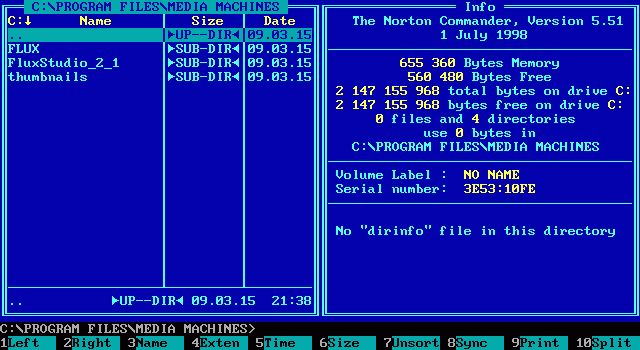
\includegraphics[width=0.7\hsize]{NortonCommander.png}
}

\only<2> {
\begin{block} { 窗口系统 (windowing system)}
一种图形用户接口,为用户界面定义了WIMP(窗口,图标,菜单,光标)风格,提供API支持应用系统界面开发。通过使用控件工具箱可简化应用程序界面开发工作\\
例:X11,Wayland,Quartz,ExtJS
\end{block}

\begin{block}{控件工具箱(widget toolkit, widget library)}
支持图形界面开发的控件(界面元素)集,包括标签、菜单、按钮、滚动条等基本控件,以及窗口、面板等容器控件 \\
例:Motif,Mac OS X Cocoa,Windows API,QT,GTK+
\end{block}
}

\only<3> {
\begin{block}{桌面环境(Desktop Environment)}
桌面环境为系统提供了一套完整的图形用户接口,并通常集成了若干应用和工具,这些应用和工具有一致的WIMP风格和视感,基于共同的控件工具箱开发而成 \\
例:CDE,GNOME, KDE, XFCE,MS Aero,Mac OS Aqua
\end{block}
}

\only<4> {

\begin{block}{可视化编程环境}
将窗口系统、可视化开发工具、编程语言以及控件工具箱等结合为一体的可视化开发平台,支持用户以“所见即所得”的方式构造用户界面 \\
例:MS Visual Studio, NetBeans, Apple Xcode, QT Creator, App Inventor for Android 
\end{block}

}
\end{frame}

\begin{frame}
  \frametitle{人机界面的开发}
  人机界面的开发不仅是设计和实现问题,也包括分析问题
  ——对人机交互需求的分析。 \\[2ex]
  人机界面的开发也不纯粹是\textcolor{blue}{软件}问题,它还需要\textcolor{blue}{心理学}、
  \textcolor{blue}{美学}等许多其它学科的知识。 \\[2ex]

  把人机交互部分作为系统中一个独立的组成部分进行分析和设计,有利于
  \alert{隔离}界面支持系统的变化对问题域部分的影响
\end{frame}


\subsection{需求分析}

\begin{frame}
  \frametitle{人机交互部分的需求分析}
  \begin{itemize}
    \item 对使用系统的人进行分析 \\
以便设计出适合其特点的交互方式和界面表现形式
\item 对人和机器的交互过程进行分析 \\
核心问题是人如何命令系统,以及系统如何向人提交信息
\end{itemize}
\end{frame}

\begin{frame}
  \frametitle{分析与系统交互的人(参与者)}
  人对界面的需求,不仅在于人机交互的内容,而且在于他们对界面表现形式、风
  格等方面的爱好。
  前者是\textcolor{blue}{客观需求},对谁都一样;
  后者是\textcolor{blue}{主观需求},因人而异

  \begin{itemize}
    \item 列举所有的人员参与者
    \item 区分人员类型
    \item 统计(或估算)各类人员的比例
    \item 调查研究使用者的情况
    \item 了解使用者的主观需求
  \end{itemize}

\end{frame}

\begin{frame}
  \frametitle{从用况分析人机交互}
  \textcolor{blue}{用况的构成}:参与者的行为和系统行为按时间顺序交替出现
  ,左右分明,形成交叉排列的段落: \\
    \quad 每个段落至少含有一个输入语句或输出语句; \\
    \quad 有若干纯属参与者自身或系统自身的行为陈述; \\
    \quad 可能包含一些控制语句或括号。 \\

    \textcolor{blue}{抽取方法}: \\
    \quad 删除所有与输入、输出无关的语句 \\
    \quad 删除不再包含任何内容的控制语句与括号 \\
    \quad 剩下的就是对一项功能的人机交互描述
\end{frame}

\begin{frame}[fragile]
  \frametitle{示例:用况描述1}
\renewcommand\baselinestretch{1.3}
\begin{Verbatim} [commandchars=\\\{\}, label=收款用况 p1]
\textbf{收款}
输入开始本次收款的命令;
         作好收款准备,应收款总数
         置为0,输出提示信息;
for  顾客选购的每种商品 do
  输入商品编号;
  if  此种商品多于一件 then
    输入商品数量
  end if;
         检索商品名称及单价;
         货架商品数减去售出数;
\end{Verbatim}
\end{frame}

\begin{frame}[fragile]
  \frametitle{示例:用况描述2}
\renewcommand\baselinestretch{1.3}
\begin{Verbatim}[firstnumber=last, commandchars=\\\{\}, label=收款用况 p2]
        if 货架商品数低于下限 then
          通知供货员请求上货
        end if;
        计算本种商品总价并打印编号、
        名称、数量、单价、总价;
        总价累加到应收款总数;
end for;
        打印应收款总数;
输入顾客交来的款数;
        计算应找回的款数,
        打印以上两个数目,
        收款数计入账册。
\end{Verbatim}
\end{frame}

\begin{frame}[fragile]
  \frametitle{示例:去除非交互内容1}
\renewcommand\baselinestretch{1.3}
\begin{Verbatim}[commandchars=\\\{\}, label=收款用况 p1]
\textbf{收款}
输入开始本次收款的命令;
        \sout{作好收款准备,应收款总数}
        \sout{置为0},输出提示信息;
for  顾客选购的每种商品 do
  输入商品编号;
  if  此种商品多于一件 then
    输入商品数量
  end if;
        \sout{检索商品名称及单价;}
        \sout{货架商品数减去售出数;}
\end{Verbatim}
\end{frame}

\begin{frame}[fragile]
  \frametitle{示例:去除非交互内容2}
\renewcommand\baselinestretch{1.3}
\begin{Verbatim}[firstnumber=last, commandchars=\\\{\}, label=收款用况 p2]
        \sout{if  货架商品数低于下限 then}
          \sout{通知供货员请求上货}
        \sout{end if;}
        \sout{计算本种商品总价并}打印编号、
        名称、数量、单价、总价;
        \sout{总价累加到应收款总数;}
end for;
        打印应收款总数;
输入顾客交来的款数;
        \sout{计算应找回的款数,}
        打印以上两个数目,
        \sout{收款数计入账册。}
\end{Verbatim}
\end{frame}

\begin{frame}[fragile]
  \frametitle{示例:得到的人机交互描述}
\renewcommand\baselinestretch{1.2}
\begin{Verbatim}[commandchars=\\\{\}, label=收款.人机交互]
\textbf{收款员.收款(人机交互)}
输入开始本次收款的命令;
          输出提示信息;
for 顾客选购的每种商品 do
  输入商品编号;
    if 此种商品多于一件 then
      输入商品数量
    end if;
          打印商品编号、名称、数量、单价、总价;
end for;
          打印应收款总数
输入顾客交来的款数
          打印交款数及找回款数;
\end{Verbatim}
\end{frame}

\begin{frame}
  \frametitle{人机交互的细化}
  \noindent\fbox{
    \parbox{0.9\hsize} {
    \centering 输入相比输出在人机交互中起到主导作用\\
   \centering  一条输入相当于一条对系统的\alert{命令}
    }
  }\\[1ex]
  \textcolor{blue}{输入的细化}
  \begin{itemize}
    \item 输入步骤的细化
    \item 输入设备的选择
    \item 输入信息表现形式的选择
  \end{itemize}

  \textcolor{blue}{输出的细化}
  \begin{itemize}
    \item 输出步骤的细化
    \item 输出设备的选择
    \item 输出信息表现形式的选择
  \end{itemize}
\end{frame}

\begin{frame}
  \frametitle{命令的组织}
  \only<1> {
  \noindent\alert{不怎么受欢迎}的命令组织方式:
  \begin{itemize}
    \item 一条命令含有大量的参数和任选项
    \item 系统有大量命令,不加任何组织和引导
  \end{itemize}

  \noindent 命令的组织措施——分解与组合 \\
  \textcolor{blue}{分解}:将含有许多参数和选项的命令分解为若干
  \textcolor{blue}{命令步} \\
  \textcolor{blue}{组合}:将\textcolor{blue}{基本命令}组织成
  \textcolor{blue}{高层命令},从高层命令引向基本命令
  }

  \only<2> {
    \begin{block}{基本命令}
      使用一项独立的系统功能的命令
    \end{block}
    \begin{block}{命令步}    
      基本命令交互过程中所包含的具体输入步骤
    \end{block}
    \begin{block}{高层命令}
      由其他若干命令组合而成,起组织和引导作用
    \end{block}
  }
\end{frame}

\begin{frame}
  \frametitle{基本命令及其命令步的结构}

  \only<1> {
\centering
\begin{figure}
  \begin{tikzpicture}[semithick, >=stealth', shorten >=1pt, shorten <=1pt]
\graph [grow right=1.5cm, empty nodes, nodes={draw, circle, thick}] 
{ a[fill] -> b ->  c -> d -> e -> f};
\end{tikzpicture}

{线性结构}
\end{figure}

\vspace*{3ex}
\centering\begin{figure}
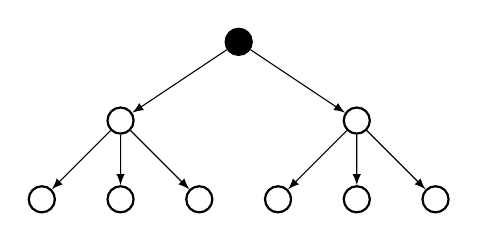
\begin{tikzpicture} [
    level distance=1cm,
    level 1/.style={sibling distance=3cm},
    level 2/.style={sibling distance=1cm},
    edge from parent/.style={draw,-latex}
  ]
  \tikzstyle{every node}=[circle,draw, thick]
  \node (Root) [fill] {}
    child {
      node {} 
        child { node {} }
        child { node {} }
        child { node {} }
    }
    child {
      node {}
        child { node {} }
        child { node {} }
        child { node {} }
    };
\end{tikzpicture}

{树形结构}
\end{figure}
}

\only<2> {
\centering\begin{figure}
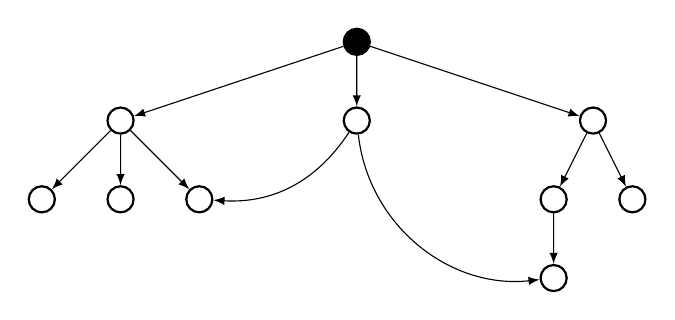
\begin{tikzpicture} [
    level distance=1cm,
    level 1/.style={sibling distance=3cm},
    level 2/.style={sibling distance=1cm},
    level 3/.style={sibling distance=0.5cm},
    edge from parent/.style={draw,-latex}
  ]
  \tikzstyle{every node}=[circle,draw, thick]
  \node (Root) [fill] {}
    child {
      node {} 
        child { node {} }
        child { node {} }
        child { node (R1) {} }
    }
    child { node (M1) {} }
    child {
      node {}
        child { 
          node {} 
            child { node (R2) {}}
          }
        child { node {} }
    };
    \draw [-latex] (M1) to [bend left=30]  (R1) ;
    \draw [-latex] (M1) to [bend right=45] (R2) ;
\end{tikzpicture}

半序网状结构
\end{figure}

}

\only<3> {
\centering\begin{figure}
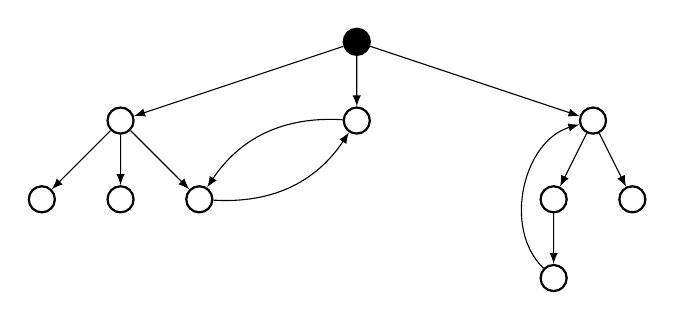
\begin{tikzpicture} [
    level distance=1cm,
    level 1/.style={sibling distance=3cm},
    level 2/.style={sibling distance=1cm},
    level 3/.style={sibling distance=0.5cm},
    edge from parent/.style={draw,-latex}
  ]
  \tikzstyle{every node}=[circle,draw, thick]
  \node (Root) [fill] {}
    child {
      node {} 
        child { node {} }
        child { node {} }
        child { node (R1) {} }
    }
    child { node (M1) {} }
    child {
      node (M2) {}
        child { 
          node {} 
            child { node (R2) {}}
          }
        child { node {} }
    };
    \draw [-latex] (M1) to [bend right=30]  (R1) ;
    \draw [-latex] (R1) to [bend right=30]  (M1) ;

    \draw [-latex] (R2) to [bend left=60] (M2) ;
\end{tikzpicture}

一般网状结构
\end{figure}

}
\end{frame}

\begin{frame}
  \frametitle{高层命令的组织结构}
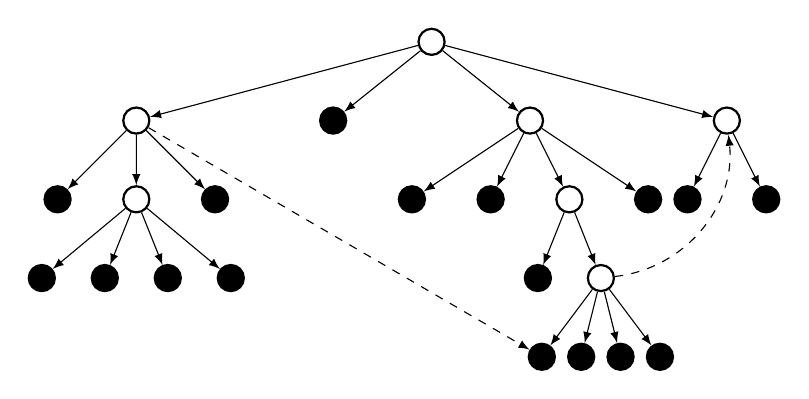
\begin{tikzpicture} [
    level distance=1cm,
    level 1/.style={sibling distance=2.5cm},
    level 2/.style={sibling distance=1cm},
    level 3/.style={sibling distance=0.8cm},
    level 4/.style={sibling distance=0.5cm},
    edge from parent/.style={draw,-latex}
  ]
  \tikzstyle{every node}=[circle,draw, thick]
  \node {}
    child {
      node (L1) {} 
        child { node [fill] {} }
        child { node (L1-1) {} 
          child { node [fill] {} }
          child { node [fill] {} }
          child { node [fill] {} }
          child { node [fill] {} }
        }
        child { node [fill] {} }
    }
    child { node [fill] {} }
    child {
      node (L2) {}
      child { node [fill] {} }
      child { node [fill] {} }
        child { 
          node {} 
            child { node [fill] {} }
            child { node (L2-1) {}
              child { node (L2-1-1) [fill] {} }
              child { node [fill] {} }
              child { node [fill] {} }
              child { node [fill] {} }
            }
          }
       child { node [fill] {} }
    }
    child {
      node (L3) {}
      child { node [fill] {} }
      child { node [fill] {} }
    };
    \draw [-latex, dashed] (L1) to  (L2-1-1) ;
    \draw [-latex, dashed] (L2-1) to [bend right=45] (L3) ;
\end{tikzpicture}

\end{frame}

\begin{frame}
  \frametitle{输出信息的组织结构}
  \only<1> {
\centering\begin{figure}
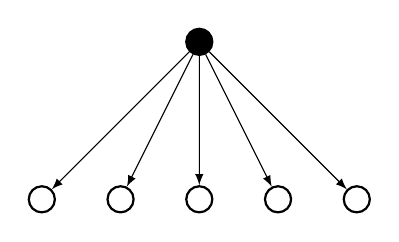
\begin{tikzpicture} [
    level distance=2cm,
    level 1/.style={sibling distance=1cm},
    edge from parent/.style={draw,-latex}
  ]
  \tikzstyle{every node}=[circle,draw, thick]
  \node (Root) [fill] {}
        child { node {} }
        child { node {} }
        child { node {} }
        child { node {} }
        child { node {} } ;
\end{tikzpicture}

两层命令
\end{figure}

  }

  \only<2> {

    \centering\begin{figure}
  \begin{tikzpicture}[node distance=0.8cm]
    \tikzstyle{decision} = [diamond, draw, 
      text width=3em, text centered, inner sep=0pt]
    \tikzstyle{block} = [rectangle, draw, 
      text width=5em, text centered, rounded corners, minimum height=2em]
    \tikzstyle{line} = [draw, very thick, color=black!50, -latex']
    \tikzstyle{line2} = [line, shorten <=5pt]

    \node [circle, draw] (init) {} ;
    \node [block, below = of init] (feed) {反馈信息};
    \node [block, below = of feed] (deal) {处理结果};
    \node [block, below = of deal] (promp) {提示信息};
    \path [line] (init) -- (feed);
    \path [line] (feed) -- (deal);
    \path [line] (deal) -- (promp);

    \path [line] ($(init.south) ! 0.5 ! (feed.north) $) -- ++(-2, 0) |- 
      ($ (feed.south) ! 0.5 ! (deal.north) $) ;
    \path [line] ($(init.south) ! 0.5 ! (feed.north) $) -- ++(-2, 0) |- 
      ($ (deal.south) ! 0.5 ! (promp.north) $) ;

    \node [circle, draw, below= of promp] (o0) {} ;
    \node [circle, draw, right= 0.6 of o0] (r1) {} ;
    \node [circle, draw, right= 0.6 of r1] (r2) {} ;
    \node [circle, draw, right= 0.6 of r2] (r3) {} ;
    \node [circle, draw, left= 0.6 of o0] (l1) {} ;
    \node [circle, draw, left= 0.6 of l1] (l2) {} ;
    \node [circle, draw, left= 0.6 of l2] (l3) {} ;
    \path [line2] (promp) -- (l3) ;
    \path [line2] (promp) -- (l2) ;
    \path [line2] (promp) -- (l1) ;
    \path [line2] (promp) -- (o0) ;
    \path [line2] (promp) -- (r1) ;
    \path [line2] (promp) -- (r2) ;
    \path [line2] (promp) -- (r3) ;
  \end{tikzpicture}

    典型的输出信息结构
  \end{figure}
  }

  \only<3> {

  \centering\begin{figure}
  \scalebox{0.8} {
  \begin{tikzpicture}[node distance=0.5cm]
    \tikzstyle{decision} = [diamond, draw, aspect=2, 
      text width=3em, text centered, inner sep=0pt]
    \tikzstyle{block} = [rectangle, draw, 
      text width=5em, text centered, rounded corners, minimum height=1.5em]
    \tikzstyle{line} = [draw, very thick, color=black!50, -latex']
    \tikzstyle{line2} = [line, shorten <=5pt]
    \node [circle, draw] (init) {} ;
    \node [block, below = of init] (feed1) {反馈信息};
    \node [block, below = of feed1] (deal1) {处理结果};
    \node [decision, below = of deal1] (decide1) {};
    \node [below = of decide1] (null1) {};
    \node [block, left = of null1] (deal2) {处理结果};
    \node [block, below = of deal2] (promp1) {提示信息};
    \node [decision, right = 2cm of null1] (decide2) {};
    \node [below= of decide2] (null2) {};
    \node [block, left = of null2] (promp2) {提示信息};
    \node [block, right = of null2] (deal3) {处理结果};
    \node [block, below = of deal3] (promp3) {提示信息};
    \path [line] (init) -- (feed1);
    \path [line] (feed1) -- (deal1);
    \path [line] (deal1) -- (decide1);
    \path [line] (decide1) -| (deal2);
    \path [line] (deal2) -- (promp1);
    \path [line] (decide1) -| (decide2);
    \path [line] (decide2) -| (promp2);
    \path [line] (decide2) -| (deal3);
    \path [line] (deal3) -- (promp3);

    \node [circle, draw, below=2cm of promp2] (o0) {} ;
    \node [circle, draw, right= 0.8cm of o0] (r1) {} ;
    \node [circle, draw, right= 0.8cm of r1] (r2) {} ;
    \node [circle, draw, right= 0.8cm of r2] (r3) {} ;
    \node [circle, draw, left= 0.8cm of o0] (l1) {} ;
    \node [circle, draw, left= 0.8cm of l1] (l2) {} ;
    \node [circle, draw, left= 0.8cm of l2] (l3) {} ;

    \path [line2] (promp1) -- (l1) ;
    \path [line2] (promp1) -- (l2) ;
    \path [line2] (promp1) -- (l3) ;
    \path [line2] (promp2) -- (l2) ;
    \path [line2] (promp2) -- (l1) ;
    \path [line2] (promp2) -- (o0) ;
    \path [line2] (promp2) -- (r1) ;
    \path [line2] (promp3) -- (r1) ;
    \path [line2] (promp3) -- (r2) ;
    \path [line2] (promp3) -- (r3) ;
  \end{tikzpicture}
  }

   复杂的输出信息结构
  \end{figure}
  }

\end{frame}

\subsection{人机界面设计}

\begin{frame}
\frametitle{人机界面的设计准则}
\begin{itemize}
\item 使用简便
\item 一致性
\item 启发性
\item 减少人脑记忆的负担
\item 减少重复的输入
\item 容错性
\item 及时反馈
\item 其它:\uline{艺术性}、\uline{趣味性}、\uline{风格}、\uline{视感} \ldots
\end{itemize}
\end{frame}

\begin{frame}
\frametitle{人机界面的OO设计}
\begin{itemize}
\item 选择界面支持系统
\item 根据人机交互需求选用界面元素
\item 用OO概念表示界面元素
\end{itemize}
\end{frame}



\begin{frame}
  \frametitle{选择界面支持系统}
选择界面支持系统考虑的因素:
\begin{itemize}
\item 硬件
\item 操作系统及编程语言 
\item 开发工具
\item 支持级别 
\item 风格与视感 
\item \ldots
\end{itemize}
\end{frame}

\begin{frame}
\frametitle{根据人机交互需求选用界面元素}

不同的界面支持系统提供不同的界面元素,常用的界面元素有:{窗口}、{菜单}、{对话盒}、{图符}、{滚动条}等,大多数界面元素使用\uline{事件驱动}的交互方式 \\

\begin{overlayarea}{\columnwidth}{.7\textheight}

\only<1> {
  \begin{itemize}
    \item 系统的启动
      \begin{itemize}
          \item 选用实现主界面的界面元素,如框架窗口、对话框窗口
      \end{itemize}
    \item 高层命令组织结构的实现
      \begin{itemize}
        \item 通过界面元素的构造层次体现高层命令的组织结构 \\
          \quad 例如:窗口-- 菜单-- 下级菜单 \ldots
      \end{itemize}
  \end{itemize}
}

\only<2> {
  \begin{itemize}
    \item 基本命令的执行
      \begin{itemize}
        \item 通过高层命令引向基本命令 \\
          \quad 例如:窗口—菜单—菜单选项
      \end{itemize}
    \item 详细交互过程的输入与输出
      \begin{itemize}
        \item 选择适当的界面元素完成每个命令步的输入与输出
      \end{itemize}
    \item 异常命令的输入
      \begin{itemize}
          \item 使用支持异常命令输入的界面功能,如鼠标右键菜单
      \end{itemize}
  \end{itemize}
}
\end{overlayarea}

\end{frame}

\begin{frame}
\frametitle{用OO概念表示界面元素}

\only<1> {
对象和类:尽可能使用界面类库中提供的可复用类 \\[2ex]

\begin{tikzpicture}
\umlemptyclass[type=复用, fill=white]{类库中的类名}
\umlemptyclass[fill=white, x=4]{自定义的类名}
\end{tikzpicture}
}

\only<2> {
类的属性与操作:
\begin{itemize}
\item 用属性表示界面对象的静态特征
\begin{itemize}
\item 物理特征——如:位置、尺寸、颜色、立体效果 
\item 逻辑特征——聚合、关联
\end{itemize}
\item 用操作表示界面对象的行为
\begin{itemize}
\item 例如:创建、激活、最大化、最小化、移动、选中、单击、双击 ……
\end{itemize}
\end{itemize}
}

\only<3> {
\begin{columns}
\column{0.4\hsize}

整体-部分结构:
\noindent\begin{itemize}
  \item 表示界面元素之间的构成关系,例如:
    \begin{itemize}
      \item 窗口 与 其中的菜单、按钮、图符、对话框、滚动条
    \end{itemize}
  \item 表示界面对象在操作中的逻辑层次
    \begin{itemize}
      \item 反映上、下两层命令之间的关系
    \end{itemize}
\end{itemize}

\column{0.6\hsize}
\centering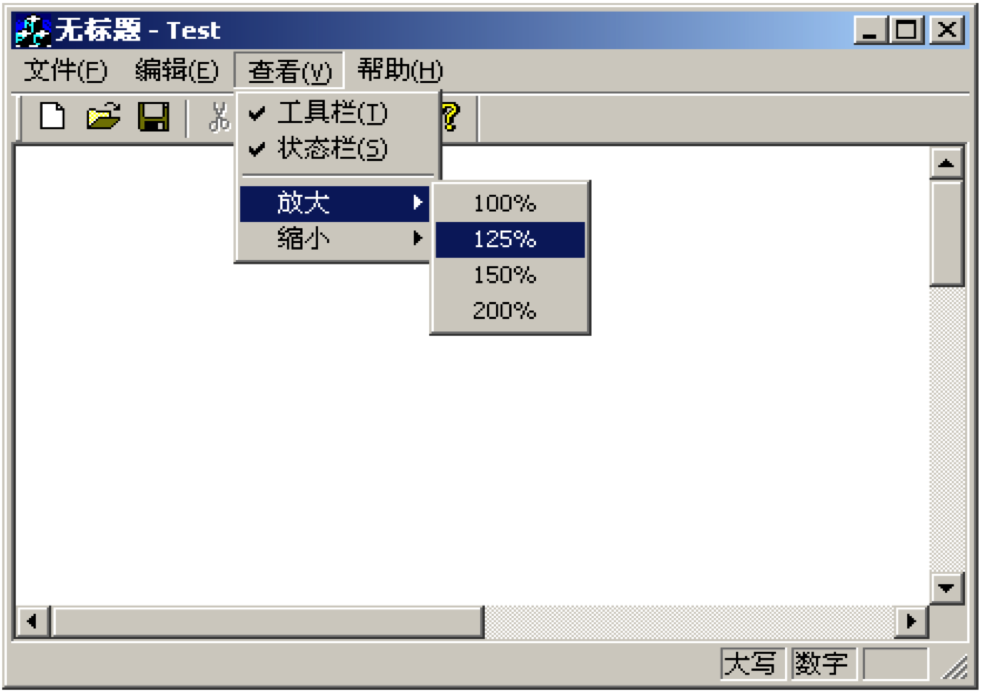
\includegraphics[width=1.0\hsize]{window.png}
\end{columns}
}

\only<4> {
整体部分结构: \\[2ex]

\scalebox{0.95}{
\begin{tikzpicture}
\tikzumlset{fill class=white}

\umlemptyclass{框架窗口}
\umlemptyclass[x=-3]{主菜单}
\umlemptyclass[x=-3, y=-2.5]{下拉菜单}
\umlemptyclass[y=-2.5]{视窗}
\umlemptyclass[y=-2.5, x=3]{工具条}
\umlemptyclass[y=-5]{滚动条}
\umlemptyclass[y=-5, x=3]{按钮}

\umlaggreg[mult1=1, mult2=1]{框架窗口}{主菜单}
\umlaggreg[mult1=1, mult2=1]{框架窗口}{视窗}
\umlHVaggreg[mult1=1, mult2=1, pos2=1.9]{框架窗口}{工具条}
\umlaggreg[mult1=1, mult2=0..2]{视窗}{滚动条}
\umlaggreg[mult1=1, mult2=*]{工具条}{按钮}
\umlaggreg[mult1=1, mult2=*]{主菜单}{下拉菜单}
\umlaggreg[mult=*, pos=0.8 , angle1=-90, angle2=-140, loopsize=2cm]{下拉菜单}{下拉菜单}
\end{tikzpicture}
}
}

\only<5> {
一般-特殊结构:
表示较一般的界面类和较特殊的界面类之间的关系  
\quad \begin{itemize}
\item 自定义的类之间的一般-特殊关系
\item 用一般-特殊结构特化可复用类
\end{itemize}

\vspace*{2ex}
\centering\begin{tikzpicture}
\tikzumlset{fill class=white}
\umlemptyclass[type=复用]{CDialog}
\umlclass[x=3]{对话框A}{属性}{操作}
\umlinherit{对话框A}{CDialog}
\end{tikzpicture}
}

\only<6> {
关联:表示界面类之间一个有特定意义的关系\\
例如: \\[3ex]
\centering\begin{tikzpicture}
\tikzumlset{fill class=white}
\umlemptyclass{工具条}
\umlemptyclass[x=3]{按钮}
\umlemptyclass[x=6]{对话框}
\umlaggreg[mult1=1, mult2=*]{工具条}{按钮}
\umlassoc[mult1=1, mult2=1]{按钮}{对话框}
\end{tikzpicture}
}

\only<7> {
消息: 
\begin{itemize}
\item 高层命令到低层命令
\begin{itemize}
\item 界面对象之间的消息
\end{itemize}
\item 基本命令的执行
\begin{itemize}
\item 从界面对象向功能对象发消息 
\end{itemize}
\item 信息输出
\begin{itemize}
\item 从功能对象向界面对象发消息
\end{itemize}
\end{itemize}
}

\end{frame}

\subsection{可视化环境下的设计}

\begin{frame}
\frametitle{可视化编程环境下的人机界面设计}
\begin{itemize}
\item 问题的提出
\item 所见即所得的界面开发
\item 设计的必要性
\item 基于可视化编程环境的设计策略
\end{itemize}
\end{frame}

\begin{frame}
\frametitle{设计的必要性}

\only<1> {
\begin{enumerate}
  \item 为实现提供依据
\begin{itemize}
\item 为了满足人机交互的需求,人机界面中要使用哪些界面对象?
\item 交互过程中的各项输入和输出应由哪些界面对象完成?

\item 如何通过界面对象类之间的各种关系体现人机交互命令的组织结构与层次?
\item 如何通过界面对象和功能对象之间的消息实现它们之间的动态联系?
\end{itemize}
\end{enumerate}
}

\only<2> {
  \begin{enumerate}
      \setcounter{enumi}{1}
    \item 降低失败的风险
    \item 设计和实现分离,符合软件工程良好实践经验
    \item 可视化编程环境下的设计策略有所不同
      \begin{itemize}
        \item 类库的存在促进了复用
        \item 以所见即所得的定义界面对象的各种物理属性方式更为直接
      \end{itemize}
  \end{enumerate}
}

\end{frame}


\begin{frame}
\frametitle{基于可视化编程环境的设计策略}
\begin{enumerate}
  \item 学习可视化编程环境及其类库
  \item 根据人机交互需求选择界面元素
  \item 根据可视化编程环境的特点,建立类图
\end{enumerate}
\end{frame}

\begin{frame}
  \frametitle{建立类图---做什么,不做什么}

  \only<1> {
  \textcolor{blue}{类的设立}---首先想到\uline{复用} \\[2ex]

\begin{tikzpicture}
\tikzumlset{fill class=white}

\umlemptyclass[type=复用]{CEdit}

\umlemptyclass[type=复用, x=5]{CDialog}
\umlemptyclass[x=5, y=-3]{CMyDialog}

\umlinherit{CMyDialog}{CDialog}

\node at (5, -4.2) {通过继承复用} ;
\node at (0, -4.2) {直接复用} ;
\end{tikzpicture}
}


\only<2> {
\textcolor{blue}{属性}---忽略物理特征,着重表示\uline{逻辑特征}

设计阶段\alert{不必关心}描述界面\alert{物理特征}的属性,诸如:大小、形状、位置、颜色、
边框、底纹、 图案式样、三维效果等, 由实现人员去自主处理效果更好,效率更高

以\textcolor{blue}{主要精力}定义描述界面\uline{逻辑特征}的属性 \\
\quad 表现\uline{命令的组织结构}的属性 \\
\qquad 例如:菜单类的每个选项表示什么命令 \\
\quad 表现界面元素之间\uline{组成关系}和\uline{关联的属性} \\
\qquad 例如:对话框中包含哪些控件
}

\only<3> {
  \textcolor{blue}{操作}---显式地表示从高层类\uline{继承}的操作

例: \quad\quad

\centering\begin{tikzpicture}
\tikzumlset{fill class=white}
\umlemptyclass[type=复用] {CDialog}
\umlclass[y=-3]{CMyDialog}{}{$\surd$ setDiagItemText}

\umlinherit{CMyDialog}{CDialog}
\end{tikzpicture}
}

\only<4> {
  \textcolor{blue}{整体-部分结构}---表现界面的\uline{组织结构和命令层次}

与采用其它界面支持系统的策略相同,需区分界面对象的普通属性和它的部分对象

有些组成部分被作为对象的一个\uline{普通属性} \\
\quad 例如:下拉菜单的选项,窗口的边框 \\
有些组成部分则被作为一个\uline{部分对象} \\
\quad 例如:对话框的一个下拉菜单或按钮 \\[2ex]

\textcolor{blue}{区分两种情况的依据}\\
\quad ——环境类库有没有给出这种组成部分的类定义
}

\only<5> {
  \textcolor{blue}{一般-特殊结构}---多从可复用类直接继承 \\[2ex]

\raisebox{5.5cm}{ 普通策略 }
\scalebox{0.80}{
\begin{tikzpicture}
\tikzumlset{fill class=white}

\umlemptyclass[type=复用] {对话框}
\umlemptyclass[y=-3] {对话框A}
\umlemptyclass[y=-3, x=-4, type=复用] {编辑框}
\umlemptyclass[y=-5.5] {对话框B}
\umlemptyclass[y=-5.5, x=-4, type=复用] {按钮}

%\node at (-4, 0.6) {普通策略} ;

\umlinherit{对话框A}{对话框}
\umlinherit{对话框B}{对话框A}
\umlaggreg[mult1=1, mult2=1]{对话框A}{编辑框}
\umlHVHaggreg[mult1=1, mult2=3, pos2=2.8, anchor1=210, anchor2=30]{对话框A}{按钮}
\umlaggreg[mult1=1, mult2=2]{对话框B}{按钮}
\end{tikzpicture}
}
}

\only<6> {
  \textcolor{blue}{一般-特殊结构}---多从可复用类直接继承 \\[2ex]
\noindent\raisebox{5cm}{
\parbox{2.5cm}{ 直接继承可复用类的策略}
}
\scalebox{0.70}{
\begin{tikzpicture}
\tikzumlset{fill class=white}

\umlemptyclass[type=复用] {对话框}
\umlemptyclass[x=-3, y=-3] {对话框A}
\umlemptyclass[x=3, y=-3] {对话框B}
\umlemptyclass[y=-6, x=-3, type=复用] {编辑框}
\umlemptyclass[y=-6, x=3, type=复用] {按钮}

%\node at (-4, 0.6) {普通策略} ;

\umlVHVinherit{对话框A}{对话框}
\umlVHVinherit{对话框B}{对话框}
\umlaggreg[mult1=1, mult2=1]{对话框A}{编辑框}
\umlaggreg[mult1=1, mult2=5]{对话框B}{按钮}
\umlaggreg[mult1=1, mult2=3]{对话框A}{按钮}
\umlaggreg[mult1=1, mult2=1]{对话框B}{编辑框}
\end{tikzpicture}
}
}

\only<7> {
  \textcolor{blue}{消息}---忽略自动实现的消息,注意\uline{需要编程实现}的消息
\begin{itemize}
\item 界面对象接收到一个操作事件,通过它的一个操作向处理该事件的功能对象所发送的消息
\item 从功能对象向完成其输入/输出的界面对象发送的消息
\item 其它:凡是需要通过手工编程来实现的消息,都要在设计中加以表示
\end{itemize}
}

\end{frame}

\end{document}
